

%%%%%%%%%%%%%%%%%%%%%%%%%%%%%%%%%----------------------%%%%%%%%%%%%%%%%%%%%%%%%%%%%%%%%%%%

%%%%%%%%%%%%%%%%%%%%%%%%%%%%%%%%% Autora: Teresa Vargas %%%%%%%%%%%%%%%%%%%%%%%%%%%%%%%%%% Doblado al inglés: Carlos Alvear


\documentclass[letterpaper,11pt]{article}
\usepackage[utf8]{inputenc}
\usepackage[margin=1.8cm,left=2.8cm,paper=letterpaper]{geometry}
\usepackage{fullpage}
\usepackage{amssymb}
\usepackage{wrapfig}
\usepackage{multirow}
\usepackage{amsmath}
\usepackage[table]{xcolor}
\usepackage{amsfonts}
\usepackage{bigstrut}
\usepackage{multirow}
\usepackage{latexsym}
\usepackage{graphicx}
\usepackage{subfigure}
\usepackage{sectsty}
\usepackage{lipsum}
\usepackage{booktabs}
\usepackage{fancyhdr}
\usepackage{appendix} 
\usepackage{float}
\usepackage[spanish]{babel}
\usepackage{makeidx}
\usepackage[bookmarks = true, colorlinks=true, linkcolor = black, citecolor = black, menucolor = black, urlcolor = black]{hyperref} 
\usepackage[none]{hyphenat}
\usepackage{enumerate}
\usepackage[font={small}]{caption}
\usepackage{blindtext}
\usepackage{siunitx}

%%%%%%%%%%%%%%%%%%%%%Pie de pagina%%%%%%%%%%%%%%%%%%%%%%%%%%%%%%


\fancyhf{}
\fancyhead[R]{\textit{ \nouppercase{\rightmark}} }
\fancyfoot[L]{Física Experimental I}
\fancyfoot[R]{Universidad de Chile}
\fancyfoot[C]{\thepage}
\renewcommand{\headrulewidth}{1pt}
\renewcommand*{\sectionmark}[1]{\markboth{\MakeUppercase{#1}}{}}

%%%%%%%%%%%%%%%%%%%%%%Definición color%%%%%%%%%%%%%%%%%%%%%%%%%%%%%
\usepackage{color}
\definecolor{gray51}{rgb}{0.51,0.51,0.51}
\definecolor{gray71}{rgb}{0.71,0.71,0.71}
\newcommand{\HRule}{\rule{\linewidth}{.4mm}}

\usepackage{listings}
\lstset{
	tabsize=4,
	language=Octave,
        basicstyle=\scriptsize,
        %upquote=true,
        aboveskip={1.5\baselineskip},
        columns=fixed,
	numbers=left,
        showstringspaces=false,
        extendedchars=true,
        breaklines=true,
        prebreak = \raisebox{0ex}[0ex][0ex]{\ensuremath{\hookleftarrow}},
	frame=false,
        showtabs=false,
        showspaces=false,
        showstringspaces=false,
        identifierstyle=\ttfamily,
        keywordstyle=\color[rgb]{0,0,1},
        commentstyle=\color[rgb]{0.133,0.545,0.133},
        stringstyle=\color[rgb]{0.627,0.126,0.941},
%	language=matlab
}


\begin{document}

%%%%%%%%%%%%%%%% Cambio nombres predeterminados%%%%%%%%%%%%%%%%%%%%%
\renewcommand{\tablename}{Tabla}
\renewcommand{\figurename}{Figura}
\renewcommand{\contentsname}{Índice}
\renewcommand{\listtablename}{Índice de tablas}
\renewcommand{\appendixname}{Anexo}
\renewcommand{\appendixtocname}{Anexos}
\renewcommand{\appendixpagename}{Anexos}


%%%%%%%%%%%%%%%%%%%%%%%%%%Inclusión portada%%%%%%%%%%%%%%%%%%%%%%%%

	\oddsidemargin 0cm \topmargin -2cm \textheight 21cm \textwidth
	16.5cm \headheight 1cm \linespread {1.0} \headsep 1cm \parindent 0mm

	\begin{titlepage}

% Upper part of the page


\includegraphics[width=4.7cm]{logo.png} 
	\hspace{0cm}
\begin{tabular}{l}
\textsc{\color{red}Departmento de Física}\\
\textsc{\color{gray51}Facultad de Ciencias Físicas y Matemáticas}\\
\textsc{\color{gray51}Universidad de Chile}\\
\textsc{\color{gray51}FI3003-1 Física Experimental I}\\
  \vspace*{1.1cm}\mbox{}
  \end{tabular}
\vspace*{2.5 cm}
  
% Titulo
\begin{center}
~\\[0.5cm]
{\color{gray71}\textsc{Física Experimental I}}
\HRule~ \\[0.4cm]
{ \Huge \textup \bfseries  Bitácora}\\[0.4cm]
{ \Large \textup{Grupo 10 }}\\[0.2cm]
\HRule ~\\[1cm]
\end{center}
\begin{minipage}{.5\textwidth}
~
\end{minipage}
\begin{minipage}{.5\textwidth}
\begin{flushright}
\vspace{.5cm}%opcional
\begin{tabular}{l}

\emph{\textbf{Integrantes}:}\\
{\small Amaru Moya}\\[.2cm]
{\small Joaquín López}\\[.2cm]


\emph{\textbf{Profesor}:} \\ 
{\small María L. Cordero}\\[0.2 cm]
{\small Victor Fuenzalida }\\[0.2 cm]

\emph{\textbf{Auxiliares}:} \\
{\small	Fernando Vergara}\\[0.2cm]
{\small	Consuelo Contreras}\\[0.2cm]

\emph{Entrega:}\\
{\small \today}
\end{tabular}
\end{flushright}
\end{minipage}
\end{titlepage}



%\end{document}

	\topmargin 0cm
	\pagestyle{empty}
	\pagestyle{fancy}
	\pagenumbering{arabic}

%%%%%%%%%%%%%%%%%%%%Espacio después del párrafo y sangrías%%%%%%%%%%%%%%%%%%%%
\setlength{\parskip}{8pt}
\setlength{\parindent}{12pt}


%%%%%%%%%%%%%%%%%%%%%%%%%%Comienzo informe%%%%%%%%%%%%%%%%%%%%%%%%
\section*{Resumen}

El siguiente documento tiene la finalidad de registrar todo material investigado para el ramo FI3003-1 :Física Experimental I 



\newpage



\begin{center}
\tableofcontents
\end{center}
\newpage


%%%Lista de Figuras
\addcontentsline{toc}{section}{Índice de figuras} %agrega índice de %figuras al índice
\begin{center}
\listoffigures
\end{center}
\newpage

%%%Lista de tablas
\addcontentsline{toc}{section}{Índice de tablas} %agrega índice de tablas %al índice
\begin{center}
\listoftables
\end{center}
\newpage

%\section{Introduction}
%
%%\subsection{Objetivo general}
%
%%\subsection{Objetivos particulares}
%
%\newpage

\section{Unidad 2: Tecnología del Vacío}

\subsection{Seguridad}

[27/08/2021  12:50]

\textbf{1) ¿Qué es el fuego? Explique en términos químicos.}

El fuego es una reacción de oxidación exotérmica, donde energía en forma de calor y luz es liberada. Este tipo de reacciones se conocen como combustiones y ocurren cuando un combustible reacciona con oxigeno (comburente) tras recibir cierta cantidad mínima de energía. Por ejemplo, si átomos de carbono y de oxigeno se acercan lo suficiente harán combustión. Debido a la repulsión electromagnética de las moléculas es necesaria cierta energía cinética mínima para superar esta barrera entre ambas partículas, la cual una vez superada da lugar a la combustión. Los productos                 resultantes tendrán más energía cinética debido al carácter exotérmico, estos productos pueden ceder energía mediante colisiones al resto de partículas circundantes lo que eventualmente puede causar una reacción en cadena que conocemos como fuego.

% Feynman Fire: https://www.youtube.com/watch?v=N1pIYI5JQLE
%https://www.aimecuador.org/documentos/capacitacion/presentaciones-varios/7-clases-fuegos/file.html
%https://es.wikipedia.org/wiki/Fuego#Comportamiento_fisicoqu%C3%ADmico
%https://www.fio.unicen.edu.ar/usuario/segumar/Laura/material/Qu%EDmica%20del%20Fuego.pdf
%https://www.scielo.cl/scielo.php?script=sci_arttext&pid=S0718-07642010000100004

\textbf{2) Investigue:}

\textbf{a) ¿Son sinónimos fuego y llama?}
No lo son; Una llama se produce en el punto de ignición de la combustión y es la parte gaseosa y visible de un fuego. Estas consisten principalmente es dióxido de carbono, vapor de agua, oxígeno y nitrógeno. Si están lo suficientemente calientes, los gases pueden ionizarse y convertirse en plasma.

\textbf{b) ¿Puede haber fuego sin llama? Proporcione un ejemplo.}

El fenómeno de combustión sin llama se presenta cuando la concentración de oxígeno en una mezcla combustible es mayor del 10$\%$ y la temperatura es mayor que la de autoignición, caracterizado por la ausencia de luminosidad en la zona de reacción. 

Otra forma de tener fuego sin llama se da cuando el combustible es demasiado pesado como para producir gases, un ejemplo es la combustión del hierro la cual no produce llama, un ejemplo más cotidiano es cuando hacemos un asado y se espera hasta que el carbón deje de producir llamas para recién poner la carne a la parrilla.

\textbf{3) Los bomberos (quienes no necesariamente poseen conocimientos de química) suelen usar los conceptos de:}

\textbf{a) Triángulo del fuego : }
El fuego se representa con un triángulo, en donde cada lado representa a uno de los componentes que deben estar presentes para la existencia del fuego. Estos son combustible, oxigeno y calor/fuente de ignición. Sin alguno de estos componentes el fuego no puede existir, ya que para esto es necesario un calor inicial y constante implica que si se destruye de cualquier manera el triángulo (eliminándolo o acortando uno de sus lados) el fuego se extingue.


\begin{figure}[H]
\centering
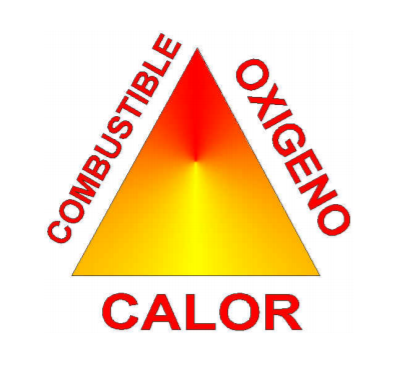
\includegraphics[scale=0.6]{triangulo de fuego.PNG} 
\caption{Triángulo de fuego.}
\label{fig:fig1}
\end{figure}


\textbf{b)Tetraedro del fuego : }Existen una serie de especies activas que son responsables de las reacciones químicas que se producen en dicho frente. Por consiguiente una nueva representación es agregar al triángulo un cuarto elemento, que será la Reacción química o en cadena, formándose un tetraedro.

\begin{figure}[H]
\centering
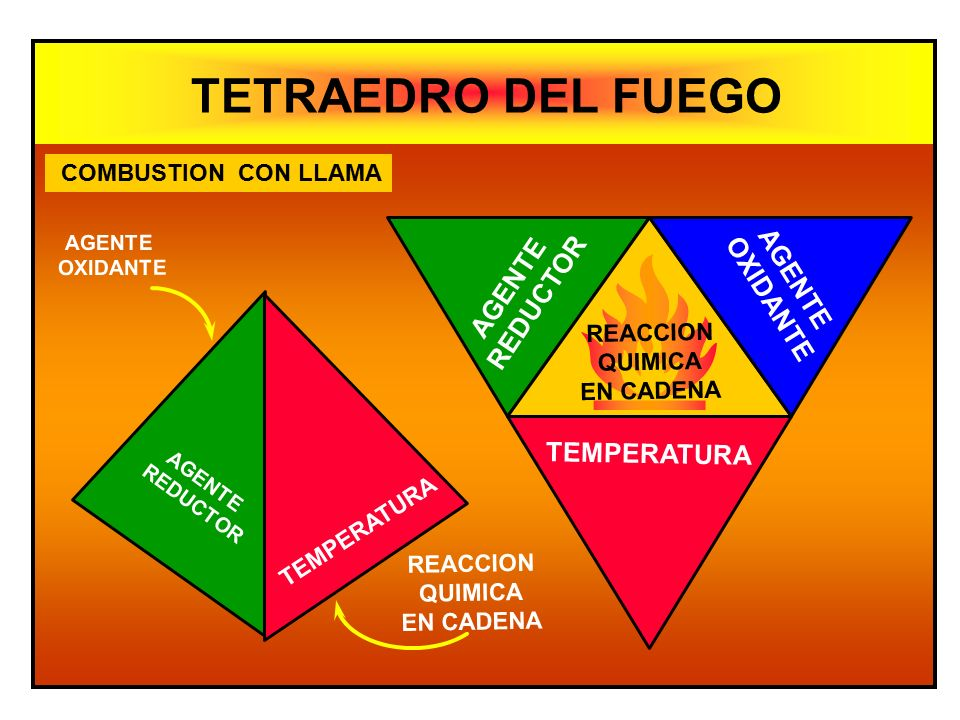
\includegraphics[scale=0.4]{TETRAEDRO+DEL+FUEGO+AGENTE+REDUCTOR+OXIDANTE+TEMPERATURA.jpg} 
\caption{tetraedro de fuego.}
\label{fig:fig2}
\end{figure}


Si la concentración de oxígeno presente desciende del 14\%, la combustión no se produce.


\textbf{4) Muestre cómo esos conceptos pueden usarse para prevenir incendios.}

El calor permite al fuego expandirse removiendo la humedad del combustible circundante, calentando el aire y precalentando el combustible en su camino. Cuando la reacción se ve limitada por el combustible, es decir, que no hay suficiente de este o cuando la ventilación es limitante, es decir, que no hay suficiente oxigeno para mantener la combustión, entonces el fuego decae a un estado de ardor más lento.

Formas de apagar un fuego:

\begin{itemize}
	\item Enfriar el combustible.
	
	\item Remover el oxigeno.
	
	\item Remover el combustible.
	
	\item Romper la reacción química.
	
	\item En caso de líquidos evitar su evaporación
	
\end{itemize}


\textbf{5) ¿Qué son los fuegos o incendios de tipo:}

\begin{wrapfigure}{l}{0.25\textwidth}
	\centering
	
\includegraphics[width=0.111\textwidth]{ABCD.png}
\end{wrapfigure}

Fuego tipo A:

Son fuegos de combustibles comunes, tales como madera, papel, géneros, cauchos y diversos plásticos.


Fuego tipo B:

Son fuegos en líquidos inflamables, aceites, grasas, alquitranes, pinturas a base de aceite, lacas y gases inflamables.



Fuego tipo C:

Son fuegos que involucran equipo eléctrico energizado, donde es importante la no conductividad eléctrica del agente de extinción (cuando el equipo eléctrico es desenergizado se puede utilizar con seguridad extintores de Clase A y B).


Fuego tipo D:

Son fuegos en metales combustibles, tales como magnesio, titanio, zirconio, sodio, litio y potasio, que al arder alcanzan temperaturas muy elevadas (2700 a 3300 Cº)


\textbf{6) Explique qué son las temperaturas de:}
\begin{itemize}
	
    \item Gasificación:
    
     Se llama Temperatura de Gasificación o Flash Point, a la temperatura mínima a la cual un combustible emana vapores en cantidad suficiente como para formar una mezcla inflamable con un comburente. Se entiende por mezcla inflamable aquella en la cual el comburente y el combustible gasificado están en proporciones que permiten la combustión.
    
    Ejemplo: La temperatura de gasificación del Keroseno es de 37,8 °C, lo que significa que para que este producto comience a emanar vapores, en cantidad suficiente para arder, debe adquirir una temperatura de 37,8 grados C., en tanto que la gasolina, a los -42,75 °C ya los comienza a desprender, por lo que a una temperatura ambiente, de 18 a 20 grados, el keroseno debe ser calentado para producir este fenómeno, mientras tanto que la gasolina ya lo está haciendo a esa temperatura.
    
    Por lo anterior, se debe considerar que mientras menor sea la temperatura de gasificación del combustible, mayor será el riesgo de incendio.
    
    Por otra parte, sobre la base de su temperatura de gasificación los líquidos se pueden clasificar en combustibles e inflamables. Los Líquidos Combustibles requieren ser calentados para arder, mientras los Líquidos Inflamables pueden hacerlo en una tempe¬ratura ambiente normal.
    
    \item Ignición:
    
     La Temperatura de Ignición o Fire Point, corresponde a la temperatura mínima a la cual un combustible emana vapores suficientes como para, ante una fuente de ignición, se enciendan y mantengan la combustión.
    
    Continuando con el ejemplo anterior, en este caso la temperatura de ignición de la gasolina es de 456 °C, lo que significa que para encenderse, ante una fuente de ignición, sus vapores deben alcanzar esta temperatura, en cambió que el keroseno, solo necesita 37°C para que estos, en presencia de una fuente calórica, se enciendan y mantengan la combustión.
    
    Lo anterior implica, por ejemplo, en relación a las Temperaturas de Gasificación e Ignición, que el keroseno emite vapores a los 37,8 °C (Temperatura de Gasificación) y que si estos vapores encuentran un objeto a 256°C inmediatamente se inflamarán (Temperatura de Ignición).
    
    Además de la temperatura de ignición se debe hacer mención a la Temperatura de Auto-ignición la cual es la mínima temperatura requerida para que una mezcla combustible/aire se inflame, sin necesidad de que exista una llama o cualquier otra fuente de ignición presente.
    
    %http://cbsebs.cl/noticia.php?826-temperaturas-de-gasificacion-(flash-point)-de-ignicion-(fire-point)-y-de-auto-ignicion
    
\end{itemize}

\textbf{7) Investigue:}

\textbf{a) Distinga entre combustible e inflamable (use los conceptos del ítem
anterior).}

Los materiales combustibles o inflamables generarán vapores al ser expuestos a una temperatura mayor o igual a la de gasificación, los cuales pueden ser fácilmente encendidos al ser expuestos a una fuente de ignición. Es por esto que mientras menor sea la temperatura de ignición, mayor será el peligro del material. Si la temperatura de gasificación de un gas es menor a los 37.8 C, entonces este es considerado inflamable, en cambio si es mayor a 37.8 C y menor a 93.3 C se considera combustible.

\textbf{b) Proporcione un ejemplo de combustible que no sea inflamable}


El fenol tiene una temperatura de gasificación de 79 C, por lo que este puede considerarse un combustible no inflamable.

\textbf{8) Explique qué es el rango de inflamabilidad.}

El rango de inflamabilidad es una clasificación de materiales en función de su temperatura de gasificación, con la intencion de dar una idea de que tan fácil puede una inflamación ocurrir.

\begin{table}[h!]
	\begin{center}
		\caption{Rango de inflamabilidad.}
		\label{tab:table1}
		\begin{tabular}{l|c|r}
			T. de gasificación (C) & Nivel de amenaza\\
			\hline
			$>93$ & Muy baja amenaza \\
			$(66,93)$ & Amenaza moderada \\
			$(38,66)$ & Amenaza alta \\
			$(-18,38)$ & Amenaza muy alta \\
			$< -18$ & Amenaza extrema \\
		\end{tabular}
	\end{center}
\end{table}

\textbf{9) Investigue:}

\textbf{a) Explique qué es la explosión volumétrica, la que ocurre al tratar de apagar con agua un incendio que no se debe apagar de ese modo.}

Cuando se intenta apagar con agua alguna sustancia con gran capacidad calorífica (como el aceite) a alta temperatura esta aumenta rápidamente la suya, y como la ebullición del agua es a tan solo 100 C, esta se evaporará rápidamente, como es sabido cuando el agua cambia de estado a vapor aumenta su volumen, y si el cambio es abrupto este aumento de volumen también lo será, esto se conoce como explosión volumétrica.

\textbf{b) Proporcione un ejemplo domestico (existe un accidente domiciliario que se ha repetido en varias oportunidades).}

Como el agua se convierte en gas a cien grados, cuando entra en contacto con aceite muy caliente se evapora de forma súbita. Al hacerlo, el agua convertida en vapor ocupará un volumen varias veces mayor al que tenía en estado líquido y este cambio de presión provoca una explosión de la pequeña burbuja de gas, haciendo que el aceite caliente que está a su alrededor salga disparado, lo que en vez de apagar el incendio probablemente lo termine expandiendo.

%https://www.heraldo.es/noticias/sociedad/2017/11/29/por-que-salta-agua-cuando-echamos-sobre-aceite-caliente-1210777-310.html?autoref=true

%%\begin{figure}[H]
%%	\centering
%%	\includegraphics[scale=0.9]{--} 
%%	\caption{Diagrama del circuito I0, representa la corriente medida con el amperímetro A y V0 representa el voltaje medido con el voltímetro V, R1 representa la resistencia.}
%%	\label{fig:fig1}
%%\end{figure}

\subsubsection{Peligros}

Los factores de muerte en caso de incendio se describen en términos simples como:

\textbf{10) Oscuridad (¿Por qué está oscuro, cuales son los peligros asociados?)}

	Si esta oscuro la visibilidad es reducida, lo que a su vez reduce la capacidad propia de encontrar extintores, salidas de emergencia, algún botón necesario para apagar algún equipo, enchufes, etc. En general, será difícil encontrar cualquier cosa necesaria para escapar, apagar el fuego o incluso ayudar a alguien.

\textbf{11) Gases y humos (Nuevamente, ¿cuáles son los peligros?)}

Muchas combustiones emanan gases que son tóxicos para los humanos, un incendio también libera mucho humo, esto puede dañar a los pulmones, lo que eventualmente puede afectar nuestra oxigenación sobre todo a la cerebro, lo que puede causar incluso un desmayo en medio del incendio lo que definitivamente reduce las posibilidades de sobrevivirlo.

\textbf{12) Tiempo. En particular, ¿cuánto tiempo tiene para escapar del incendio?}

\textbf{13) Calor}


\subsubsection{Extintores}

Averigüe en qué consisten (qué son, por qué apagan el fuego) los extintores en base a:
\begin{itemize}
    \item Agua
    \item Dióxido de carbono
    \item Polvo quimico seco
    \item Espuma química
\end{itemize}

18) Haga una tabla de doble entrada en que cada fila corresponda a un tipo de extintor.
Las entradas de las columnas son fuegos A, B, C, y D; además de una columna F en que se indique si se puede apagar a una antorcha humana y otra G que indique si el extintor produce daños materiales (¡ojalá menores que el fuego mismo!). Llene la tabla con SI y NO según corresponda.

[29/08/2021 10:00am]

\textbf{19) ¿Cómo se apaga una persona envuelta en llamas?}
%http://www.clinicagonzalez.com/articulo/Primeros-Auxilios-Como-socorrer-a-una-persona-en-llamas-
Si la persona se está corriendo debido a que está incendiándose, deténla para que puedas actuar mejor.
Apagar el fuego de la víctima cubriéndola con una manta o algo similar, teniendo cuidado de no quemarte al hacer esto.
Hazla rodar por el piso, indícale que gire sobre su propio cuerpo, protegiéndose la cara con las manos, esta es una buena forma de apagar el fuego.
El fuego también se puede apagar utilizando agua, arena o tierra. No lo hagas con un extintor, su contenido es altamente tóxico para el ser humano.
Si la persona o tú se han incendiado el cabello cubre la cara de manera muy rápida para sofocar el fuego y retira la manta inmediatamente para evitar la inhalación de gases tóxicos.
Una vez apagado el fuego, afloja y retira las ropas que no estén adheridas a las lesiones, cuidado aquí, es importante solo retirar aquellas prendas que NO estén en las partes lesionadas.
Retira cuidadosamente los anillos, reloj, pulsera, cinturón o prendas ajustadas que compriman la zona lesionada, antes que ésta se empiece a inflamar. No retires nada que haya quedado adherido a la quemadura. No rompas las ampollas, para evitar infección y mayor incomodidad.

Lleva a la víctima a un centro médico o usa los teléfonos de emergencia para que el personal médico se encargue mejor de la situación.


20) Asegúrese de que sabe:

a) Encontrar los extintores en los laboratorios
b) Mostrar al profesor que sabe cómo operarlos.

\subsubsection{Acciones} 
21) Explique qué hacer en caso de quedarse encerrado en un incendio.

22) Explique qué (y cómo) hacer en caso de huir en un incendio.

Referencias
[1] Lecciones sobre fuego disponibles en ucursos, facilitada por el cuerpo de bomberos.
[2] Fuentes en internet

\subsection{Teórico}

Son muchas las áreas de la física experimental en que se requiere el uso de bajas presiones.
La tecnología de vacío, si bien no un fin, es un medio con el que es conveniente estar
familiarizado. La realización de un experimento en vacío requiere de:
1) Cámara de vacío propiamente tal.
2) Método de evacuación (bombas de vacío).
3) Caracterización del vacío: medidores de presión total y de presiones parciales.
4) El experimento mismo.
Esta unidad proporciona una visión somera de estos aspectos.

\subsubsection{Teoría cinética de los gases} 

Propiedades de equilibrio
En las condiciones de operación en el laboratorio, presiones menores a 105 Pa y temperaturas cercanas a 300 K, los gases pueden considerarse como ideales. Los números entre paréntesis se refieren a las secciones atingentes del libro de Ohanlon [3].

1) Coloque en su bitácora una tabla con la composición del aire atmosférico (1.1).

2) Copie o pegue una tabla con factores de conversión de presión en diferentes
unidades (1.1). Diferentes instrumentos, dependiendo del proveedor, indican las
presiones en diferentes unidades. Ud. deberá anotarlas en las unidades nativas del
instrumento para evitar errores de conversión. Posteriormente, al redactar el
informe, deben todas ser convertidas a pascales.

3) Exprese la velocidad promedio de las moléculas de un gas ideal en términos de la
temperatura (2.2.1).

4) Investigue:
a) ¿Cuál es el valor típico de esta velocidad a temperatura ambiente (considere
el gas predominante en el aire)?
b) ¿Con qué velocidad macroscópica está relacionada? Explique el motivo
físico.
Propiedades de transporte (dependen del tamaño finito de las moléculas)

5) Explique qué es la sección eficaz y proporcione su orden de magnitud para el
nitrógeno. Explique cómo la obtuvo.

6) Explique qué es el camino libre medio intermolecular (2.1.3).

7) Exprese el camino libre medio intermolecular en función de la presión, temperatura,
sección eficaz, etc. Note que este camino libre se refiere, como indica el nombre,
a colisiones intermoleculares (existen otras).

8) Grafique el camino libre medio intermolecular para el nitrógeno a temperatura
ambiente en función de la presión en el intervalo 10-10 Pa a la atmosférica.
Determine Ud. mismo si conviene usar escala lineal, semi logarítmica o logarítmica:
el objetivo de un gráfico es presentar información y extraer información cuantitativa
aproximada del mismo, son estas condiciones las que definen la escala apropiada.

9) En esta parte notará que, a alguna presión suficientemente baja, el camino libre
medio intermolecular superará las dimensiones del recipiente, en cuyo caso las
moléculas no recorrerán realmente la distancia predicha por. En este caso se lo
debe reemplazar por un camino libre efectivo, que Ud. debe:
a) definir,
b) incorporar en el gráfico anterior con línea punteada.

10) Exprese la conductividad térmica de un gas en términos de las variables apropiadas,
de modo que se pueda apreciar su dependencia con la temperatura y la presión. En
el caso del nitrógeno grafíquela bajo las mismas condiciones anteriores. Note que
debe distinguir dos regímenes: el caso en que el camino libre medio intermolecular
es sensiblemente menor que las dimensiones del recipiente, y el opuesto en que el
camino libre medio intermolecular supera las dimensiones del mismo (2.3.2).
Importante: la conductividad térmica depende del camino libre medio: ¿es o ?
Tome esto en cuenta al hacer el gráfico.
Otras propiedades

11) Explique cuál es la diferencia entre absorción y adsorción.

12) Considere un recipiente de 10 l, sobre cuyas paredes se encuentra adsorbida una
capa monomolecular de gas. Es una aproximación que subestima la cantidad de
moléculas adsorbidas, pues la adsorción ocurre en multicapas12. Suponga que el gas
adsorbido es nitrógeno y que la cámara tiene una forma regular (cubica o esférica,
para simplificar).
Calcule numéricamente el número de moléculas adsorbidas, suponiendo que el área
de cada molécula es (N2), cuyo valor numérico se introdujo en 5) (El número de moléculas adsorbidas depende de la presión, suponga aquí que siempre es una capa
monomolecular, independientemente de la presión).

13) Calcule el número de moléculas en el volumen a temperatura ambiente en función
de la presión, proporcione el valor numérico a presión ambiente.



\newpage

\section{Unidad 4: Movimiento Browniano Granular}

Se introducirá a técnicas de análisis de
imágenes. En particular se realizará el seguimiento (particle tracking velocimetry)
de una partícula macroscópica en una capa de granos vibrados, para caracterizar su dinámica difusiva, análoga al movimiento Browniano. Se publicará un video del cual se extraerán los datos.

\subsection{Seguridad}
[24/08/2021  11:03 am]

\textbf{1) Averigüe que es un MSDS (Hoja de Datos de Seguridad de Materiales). ¿Para qué sirve?}

Es un documento que permite comunicar los peligros de los productos químicos para el ser humano, la infraestructura y los ecosistemas. También informa acerca de las precauciones requeridas y las medidas a tomar en casos de emergencia.
%*una MSDS es diferente de una “ficha técnica” ya que ésta tiene mayor información acerca de las especificaciones exactas e
instrucciones para el uso del producto. 

\textbf{2) Busque dos ejemplos de MSDS para fluidos que Ud. puede usar en el laboratorio.}

\href{https://quimicauniversal.cl/www/wp-content/uploads/2020/08/AGUARRAS-18-min.pdf}{uno}

\href{https://www.carlroth.com/medias/SDB-4309-ES-ES.pdf?context=bWFzdGVyfHNlY3VyaXR5RGF0YXNoZWV0c3wxNzYxNDR8YXBwbGljYXRpb24vcGRmfHNlY3VyaXR5RGF0YXNoZWV0cy9oNDEvaDMyLzg5NTA4ODUyNTMxNTAucGRmfDNlNjhiMGU1ODA0YTBmZTQ2MTdhYmQxNmU1OTAxY2UzNmNiNGQ0YTdiOGVjNWRjOGI2N2ZkNzE0MTk1ODRkZjQ}{dos}

\textbf{3) ¿Cuáles son las categorías que Ud. encontrará en el MSDS?}
\begin{enumerate}
    \item Producto e Identificación de la Compañía.
    \item Identificación de peligros.
    \item Composición, Información sobre ingredientes.
    \item Medidas de primeros auxilios.
    \item Medidas en caso de incendio.
    \item Medidas en caso de vertido accidental.
    \item Manejo y Almacenamiento.
    \item Controles de exposición y protección personal.
    \item Propiedades físicas y químicas.
    \item Estabilidad y reactividad.
    \item  Información toxicológica.
    \item Información ecológica.
    \item Consideraciones de Disposición.
    \item Información sobre transporte.
    \item Información reglamentaria.
    \item Información adicional.
\end{enumerate}
 
\textbf{4) Incluya en su bitácora los diferentes pictogramas de seguridad que indican los riesgos de una sustancia química.}
\begin{figure}[H]
	\centering
	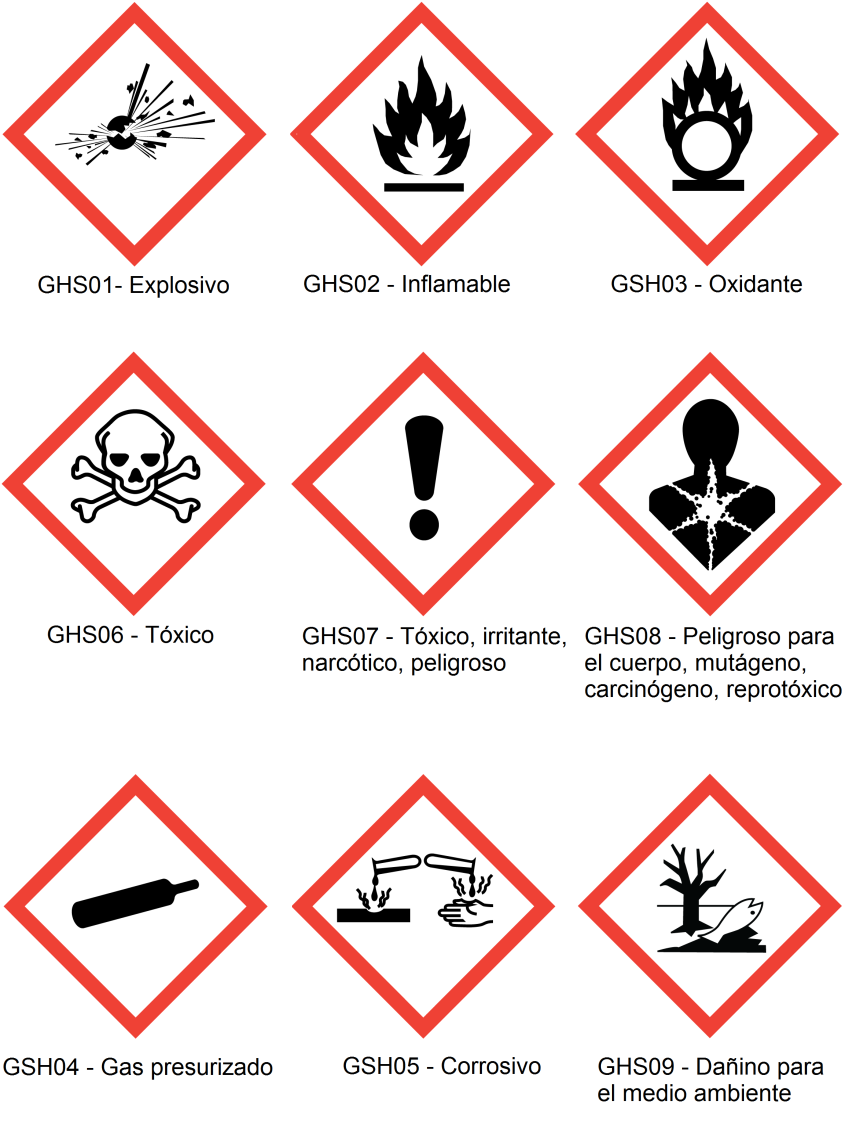
\includegraphics[scale=0.3]{pictogramas-de-seguridad.png} 
	\caption{Pictogramas de seguridad}
	\label{fig:picto1}
\end{figure}

[25/08/2021 09:45 am]

\textbf{5) Explique los protocolos requeridos para almacenar sustancias químicas.}

\url{https://www.bcn.cl/leychile/navegar?idNorma=1088802}

\textbf{6) Averigüe sobre dos fuentes confiables, una en papel y la otra digital, sobre propiedades termofísicas de al menos tres fluidos más comunes usados en el LMFE (Laboratorio de Materia Fuera del Equilibrio).}


\textbf{7) Busque los valores nominales de la densidad y tensión superficial del agua.}
Densidad: $\SI{997}{kg/m^3}$ a $\SI{298.15}{K}$ \\
Tensión superficial: $ \SI{0.07199}{N/m} $

\textbf{8) Averigüe el valor de resistividad y permitividad eléctrica del agua de la llave, de agua destilada y de agua des-ionizada.}\\
A $\SI{293.15}{K}$ 
\begin{table}[H]
\centering
\caption{Tabla de valores encontrados}
\begin{tabular}{|l|l|l|}
\hline
Tipo              & Conductividad {[}S/m{]} & Resistividad {[}\textbackslash{}Omega m \\ \hline
Agua de la llave  & 0.0005 - 0.05           & 200 - 2.000                             \\ \hline
Agua destilada    & 0.00005                 & 500.000                                 \\ \hline
Agua des-ionizada & 0.000042                & 180.000                                 \\ \hline
\end{tabular}
\label{tab:tab1a} 
\end{table}

REFERENCIAS
[1] Edward A. Lacy, Handbook of Electronic and Safety Procedures, Capítulo 9 “Toxic
and explosive chemicals”, (Prentice-Hall, Inc., New Jersey, 1977).
[2] Wikipedia
[3] Biblioteca del congreso nacional de Chile
%pa el 8
\url{https://www.ugr.es/~zoom/tablasOoM/Resistividad_Electrica.pdf}
\url{https://pubs.acs.org/doi/10.1021/jp045975a}



\subsection{Teórico}
\subsection{Imágenes digitales}
\textbf{1) Enumere y describa las características de una imagen digital.}\\


\textbf{2) Averigüe 3 modelos de cámaras disponibles en el DFI. Estas deben ser cámaras que sean usadas para diferentes situaciones físicas (escalas espaciales y/o temporales).
Indique sus características básicas y dé una breve descripción para qué son usadas.} \\ 
\url{https://www.phantomhighspeed.com}
\url{https://www.thorlabs.com/newgrouppage9.cfm?objectgroup_id=3483}
%⦁	Phantom v641: Es usada para aplicaciones de alta resolución y alta sensibilidad. Es una cámara de alta velocidad que permite capturar muchos fotogramas por segundo (fps), lo cual permite visualizar situaciones que son imperceptibles para el ojo humano. De esta forma, es una cámara con la que se pueden analizar procesos físicos que a simple vista no se pueden ver. Es ideal para aplicaciones PIV (velocimetría de imágenes de partícula: método óptico de visualización de flujo utilizado en investigación. Se usa para obtener mediciones de ⦁	velocidad instantáneas y propiedades relacionadas en ⦁	fluidos).
%⦁	Cámara con sensor CMOS de 4 Mpx.
%⦁	Rendimiento superior a 6 Gpx/seg.
%⦁	En formato full HD (1920x1080), supera los 2.500 fps.
%⦁	A una resolución completa  (2560x1600) alcanza los 1450 fps.

%⦁	Cámara MotionPro x3: Es una cámara rápida que se utiliza desde áreas como balística y aeronáutica hasta test de detección de temperatura de resistencia. 
%⦁	Resolución: 1.3 Mpx.
%⦁	Máxima resolución: 1000 fps (1280 x 1024 px) 
%⦁	resolución 512 x 512 a 5000 fps
%⦁	A color y monócroma

%⦁	Zyla andor 4.2: Es una cámara ultra-rápida que posee una sensibilidad y rapidez ideal para ser utilizada en experimentos con imágenes de calcio, microscopía de lámina de luz y microscopía de superresolución. También se usa en el área de astronomía. Para microscopios.
%⦁	Cámara de 4.2 Mpx (2048 x 2048 px)
%⦁	Hasta 27000 fps
%⦁	99.8% de linealidad
%⦁	Tecnología de sensores sCMOS
%⦁	Velocidades de fotogramas más rápidas


\textbf{3) Enumere, describa y practique operaciones básicas con imágenes usando Matlab
(abrir, visualizar, grabar, filtrar, convertir de color a escala de grises, convertir a imagen binaria usando un valor umbral).}\\

\textbf{4) Averigüe sobre métodos de seguimiento de partículas (tracking, en inglés).}\\


III. Referencias
1. Tracker: http://physlets.org/tracker/
2. ImageJ: http://rsbweb.nih.gov/ij/
3. Detección y seguimiento de partículas usando Matlab:
http://physics.georgetown.edu/matlab/ 














\newpage

%%%%%%%%%%%%%%%%%%%%%%Bibliografia%%%%%%%%%%%%%%%%%%%%%%%%%%%%%%%%%%

\bibliographystyle{ieeetr}
\bibliography{biblio}
\newpage

%%%%%%%%%%%%%%%%%%%%Anexos%%%%%%%%%%%%%%%%%%%%%%%%%%%%%%%%%%%%%%%%%%
%\appendix
%\addappheadtotoc %agrega anexos al índice
%\appendixpage
%\section{Ejemplo Anexo}


\end{document}